\section*{6.4 Efficient Parallelization of AlphaBeta}

\subsection*{1.}
In the lecture, most of those questions were already answered. A minimal tree looks like that: Every node (=move) has several children. It always has to evaluate the leftmost child in order to get initial values. Also, their values are assumed to be the best, as they represent the best moves. A leftmost child is therefore called ``all node'', because the depthsearch has to descent in every single child of them. Other nodes are then called ``cut nodes''. The process still has to descent into them, as they are children of ``all nodes'', but all of their children (minus the leftmost of them, which again is an ``all node'', can, and if the assumptions that the moves are perfectly ordered hold, will be pruned. Slides 5 to 7 of the presentation of the lecture show how such a tree looks like in picture.
A decomposition strategy presented in the lecture (and used in this task) is pvsplit, which uses somewhat a bottom up approach: First, the tree is traversed down along the principal variation, until the depthsearch reaches the maximum depth. At this point, all children of this node are evaluated by the worker processes, and their values is returned to the master. After that, the main process traverses up one step, and again distributes the work on the children of that node to the workers. However, it already knows the value of the leftmost child, as this was already evaluated in the previous step, and therefore searchoverhead should be reduced. This is repeated until the algorithm reaches the topmost layer of the tree and has evaluated the children of the root node (which obviously is also an all node, as the current boardposition is included in the best movesequence). By doing this, we can assure that we never will start depthsearch with a broad window on too many processes, and therefore should reduce search overhead significantly.
As you can see in the table, pvsplit even survives the misprediction of the alphabeta window in position-endgame without causing horrible amounts of overhead.
\begin{center}
  \begin{tabular}{|r|r|r|r|}
    \hline
    Setting & AlphaBeta & Overhead simple par (4p)& Overhead pvsplit (4p)\\ \hline
    midgame1, depth5 & 4,120,198 & 19.5\% & 18.4\%  \\ \hline
    midgame2, depth5 & 2,067,878 & 29.6\% & 13.6\%   \\ \hline
    endgame, depth5 & 402,920 & 300.1\% & 8.3\%   \\ \hline
  \end{tabular}
\end{center}


\subsection*{2. Speedup figures}
In this setting, we are using the runtime of the evaluation of the sequential version distributed to the students as a baseline, and then compare this to the runtime of our parallelization. Note that you should not use evalrate to determine speedup, because you might have (more precisely: do have) search overhead, and this would make your parallelization look a lot better than it actually is.
You can see that the parallelization does a pretty decent job, although the speedup by no means is perfect. 

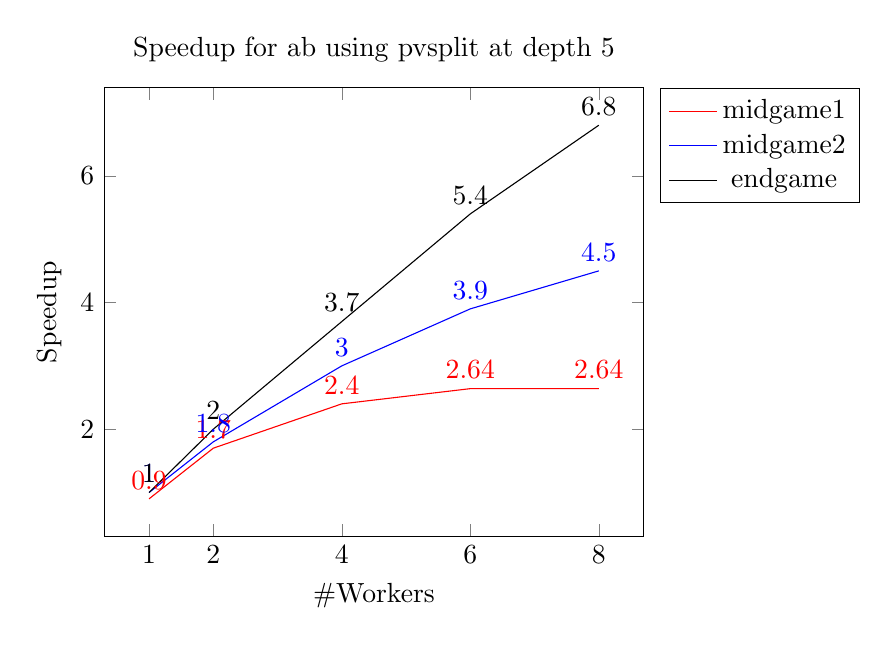
\begin{tikzpicture}
  \begin{axis}[
      legend style={cells={align=left}},
      xtick={1, 2, 4, 6, 8},
      xlabel=\#Workers,
      ylabel=Speedup,
      title=Speedup for ab using pvsplit at depth 5,
      legend pos = outer north east,
      nodes near coords,
      scaled ticks = false,
      y tick label style={
        /pgf/number format/.cd,
	fixed,
        fixed zerofill,
	precision=0,
        /tikz/.cd
      },
      no markers]
     \addplot[color=red] coordinates {
       (1,0.9)
       (2,1.7)
       (4,2.4)
       (6,2.64)
       (8,2.64)
     };
     \addplot[color=blue] coordinates {
       (1,1)
       (2,1.8)
       (4,3)
       (6,3.9)
       (8,4.5)
     };
     \addplot[color=black] coordinates {
       (1,1.0)
       (2,2)
       (4,3.7)
       (6,5.4)
       (8,6.8)
     };
     \legend{midgame1, midgame2, endgame}
  \end{axis}
  
\end{tikzpicture}
